One of the main challenges in developing the software was selecting the right programming language. As mentioned previously$^{\ref{software-objectives}}$, I needed the software to be both high-performing and flexible. A compiled language was essential, as a scripting language wouldn’t be able to handle the rendering of complex widgets, especially when trying to push the limited power of the Raspberry Pi to its limits. This led to the immediate exclusion of languages like Python and JavaScript. Although C and C++ were obvious choices due to their efficiency, I initially sought something more modern and sophisticated. However, after some experimentation, I found that the .NET runtime wasn’t suitable for the Pi, and alternatives like Java and Rust didn’t provide the same performance gains I achieved with C++ that in the end emerged as the best option.

\section{C++ Module}
I began by creating a minimal prototype capable of turning individual pixels on and off on the matrix. Fortunately, there was an excellent project on GitHub by Hzeller \footnote{\url{https://github.com/hzeller/rpi-rgb-led-matrix}} that offered a solid C++ implementation, covering the fundamental functionality I needed to get started, including: \begin{itemize} \item Direct manipulation of individual pixel colors \item Filling the entire matrix with color \item Creating an in-memory canvas to draw on while displaying something else on the matrix, allowing for smooth transitions when swapping \item Loading .bdf fonts and converting text to pixels \end{itemize}

Given the goal of providing modularity, it made sense to define a class that each Widget could inherit from, allowing them to implement their own methods. 
Each widget is designed to encapsulate its internal workings, exposing only a single method: \textit{renderNextFrame}. Similar to a sprite in a game engine, the widget’s responsibility is simply to determine where to paint pixels in the next frame—no more, no less. Here’s an example of a widget that draws a simple rectangle:

\begin{minted}{c++}
class RectangleWidget : public Widget
{
    int width, height, x, y;
    Color color;
    RectangleWidget(int width, int height, int x, int y, Color color)
    {
        this.width = width;
        this.height = height;
        this.x = x;
        this.y = y;
        this.color = color;
    }

    void renderNextFrame(Canvas *canvas)
    {
        for (int i = 0; i < width; i++) {
            for (int j = 0; j < height; j++) {
                canvas->SetPixel(x+i, y+j, color.r, color.g, color.b);
            }
        }
    }
}
\end{minted}
\newpage
At this point my application is very simple but working and it looks something like this:

\begin{minted}{c++}
int main(int argc, char *argv[]) {

    Logger::logInfo("Mosaico is starting");

    // Init matrix
    RGBMatrix::Options matrix_options;
    matrix_options.rows = 64;
    matrix_options.cols = 64;
    // Other config stuff

    // Create matrix object
    RGBMatrix *matrix = RGBMatrix::CreateFromOptions(matrix_options);

    // Create a widget
    Widget runningWidget = new RectangleWidget(w,h,x,y,color);

    // Main loop
    while (true) {
        matrix->clear();
        runningWidget->renderNextFrame(matrix);
        // delay here to ensure 30Hz refresh rate
    }
}
\end{minted}
\subsection{The Canvas} As you may have noticed, the \textit{renderNextFrame} method accepts a \textit{Canvas} object as a parameter instead of directly manipulating the matrix. This approach aligns with one of the SOLID principles: \textbf{dependency inversion} \cite{dep_inv_principle}. The widgets do not need to know the specifics of the matrix; they interact with it as if it were a simple canvas to paint on. This abstraction not only simplifies the widget code but also allowed for greater flexibility as the project evolved.

\subsection{Drawables}
\label{widget_canvas_abstraction}
As I continued developing widgets, I found myself repeatedly writing similar code, particularly for drawing shapes and text. This repetition led to the creation of the \textbf{Drawable} concept—a base class that allowed me to store common shapes and figures as objects. This abstraction made it easier to create and manipulate these elements consistently across different widgets.

The \textit{Drawable} class encapsulates shared functionality such as position, color, and animation, providing a unified interface for handling visual elements. Here's a simplified structure of the \textit{Drawable} class hierarchy:

\begin{center}
  \makebox[\textwidth]{
  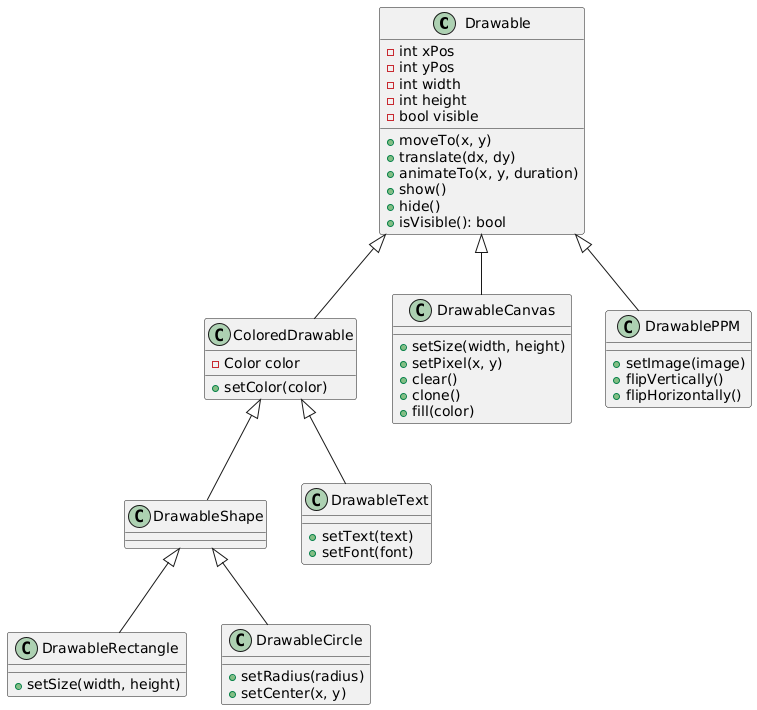
\includegraphics[width=0.8\paperwidth]{tesi/img/drawables.png}}
\end{center}

\newpage

At this point I had to edit the \textit{Widget} class in order to correctly register and render drawables.


\begin{minted}{c++}

class Widget {
private:
     // Drawables to be rendered
    std::vector<Drawable*> registeredDrawables;    
public:
    /// Add a new drawable to the widget drawable list
    void registerDrawable(Drawable* drawable);
    /// Remove a drawable from the widget drawable list
    void unregisterDrawable(Drawable* drawable);
    /// Clear all drawables
    void clearDrawables();

    void renderNextFrame(Canvas* canvas) {
        // Call the inheriting widgets to do their job
        render(canvas);
        // Drawables should be now updated, draw them
        for (Drawable* drawable : registeredDrawables) {
            drawable->draw(canvas);
        }
    }
protected:
    Widget();
    /// Pure virtual method to be overridden inheriting widgets for rendering
    virtual void render(Canvas* canvas) = 0;
};
\end{minted}

This basic setup was enough to get things up and running, enabling me to create more complex widgets.

\subsection{Loading Widgets at Runtime} At this stage, I had a straightforward method for creating new widgets and drawing shapes efficiently. If someone wanted to contribute to the project and add a new widget, they would clone the project, create a new C++ class that inherits from \textit{Widget}, write the necessary code, compile the app again, and submit a pull request.

While this approach would work, it lacked flexibility. Every time a developer added a new widget, users would need to update their software to access it. This wasn't ideal for a modular and dynamic system.

In a meeting with my supervisor, we explored the idea of treating widgets like "plug-ins" or encoded strings that the C++ program could decode in real time to display dynamic content. Although this concept was easier said than done, the potential excited me, and I immediately began experimenting with different approaches to find the best solution.

\subsubsection{Custom Encoding} My first thought was to create a custom encoding format for widgets, something akin to JSON or YAML but optimized for my needs. I imagined a frame-based system where I could specify what to render at each frame, perhaps even introducing a simple mock language to handle loops and conditionals. However, this approach proved too limiting and complex, especially for achieving the flexibility I desired. It was soon discarded.

\subsubsection{Lua vs. ChaiScript} I quickly realized that the only way to provide developers with the maximum flexibility for widget creation was to embed a Turing-complete scripting language. Drawing from my limited knowledge of game development, I knew that popular games often use Lua for custom levels and dynamic content creation \footnote{\url{https://create.roblox.com/docs/scripting}}.

Lua, being lightweight and having a C-based interpreter, seemed like a good candidate. I embedded Lua into my application, allowing it to interface with my C++ code. Initially, this appeared to be the solution, but several issues arose:

    \begin{itemize}
        \item Integration complexity: Mapping complex C++ types such as drawables, the canvas, and various helper functions to Lua proved cumbersome and overcomplicated.
        \item Syntax dissatisfaction: I found Lua's syntax unintuitive and less modern than I wanted for widget development. I aimed for a scripting language that would feel clean, readable, and enjoyable to write.
    \end{itemize}

After further research, I discovered ChaiScript \footnote{\url{https://chaiscript.com/}}, a lightweight, JavaScript-like embedded scripting language designed specifically for C++. Its integration was much simpler than Lua, with easier mapping of types and classes. I liked how the implementation was progressing, and I finally got a working solution. Below is a demo of the first widget written in ChaiScript, where I comment out parts of the code in real-time, and they are rendered immediately on the matrix!

\begin{figure}[h] \centering \begin{minipage}[b]{0.49\textwidth} \centering 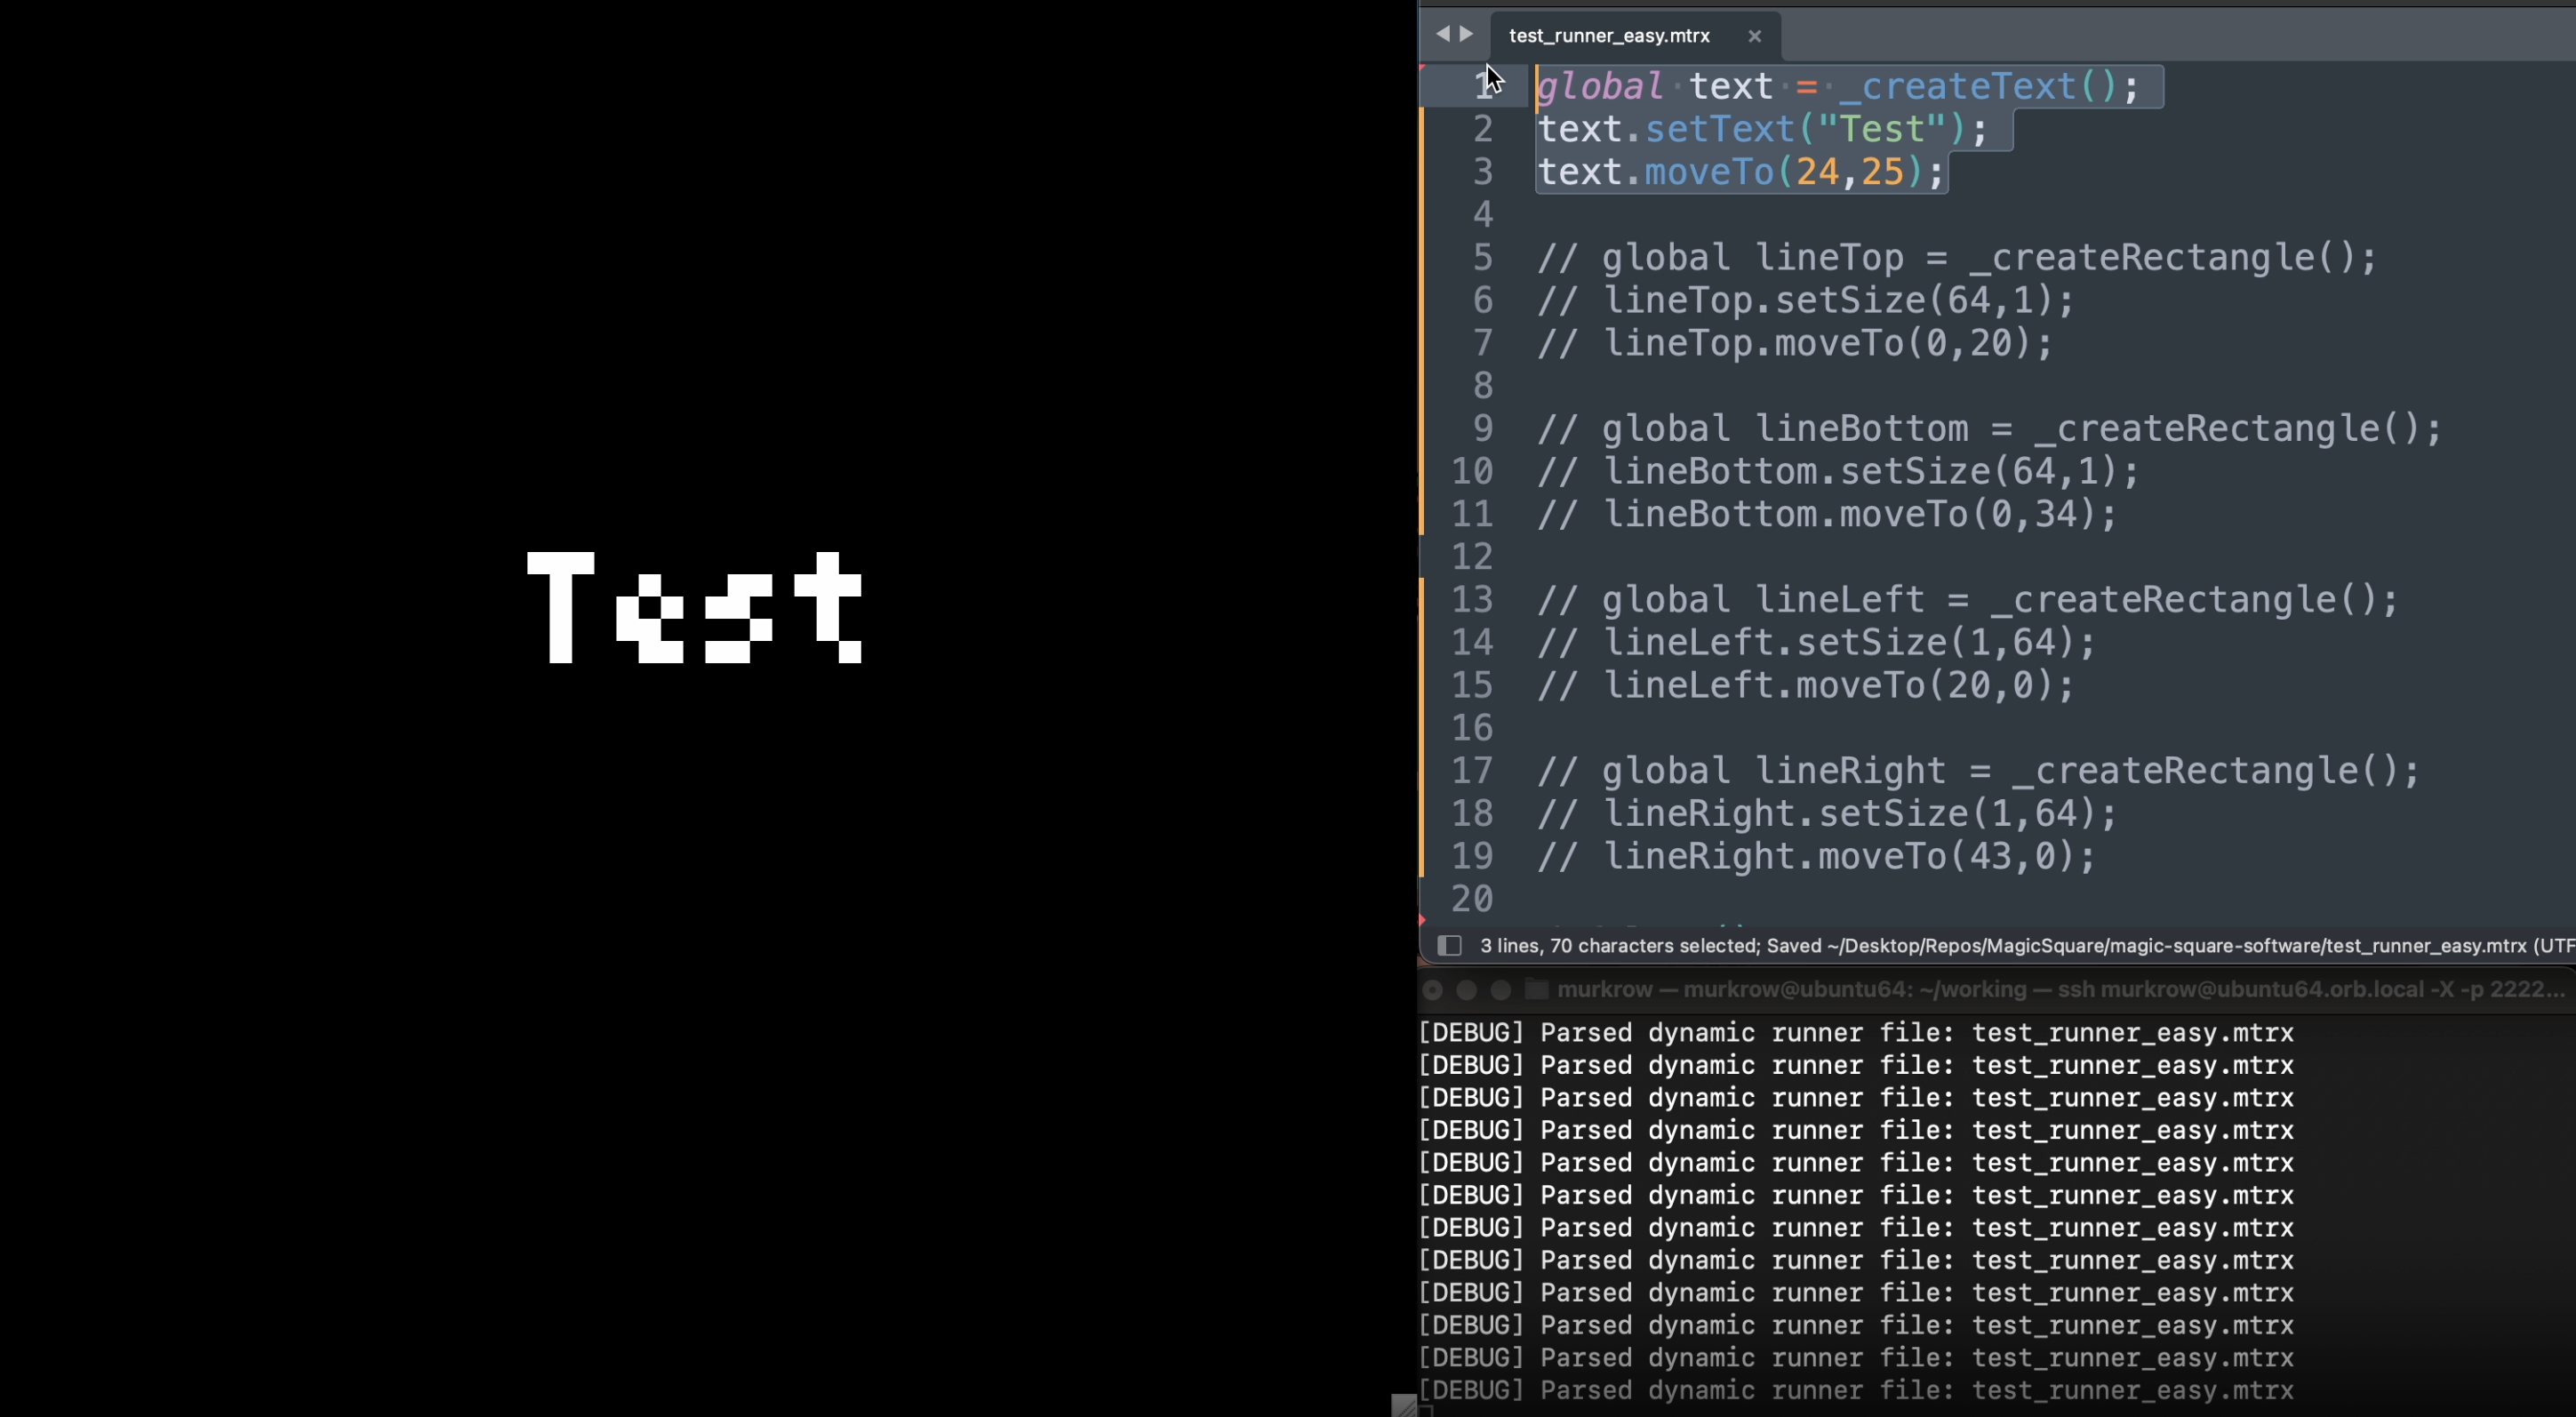
\includegraphics[width=\textwidth]{tesi/img/chai_demo/1.png} \caption*{Creation of a Text drawable} \end{minipage} \begin{minipage}[b]{0.49\textwidth} \centering 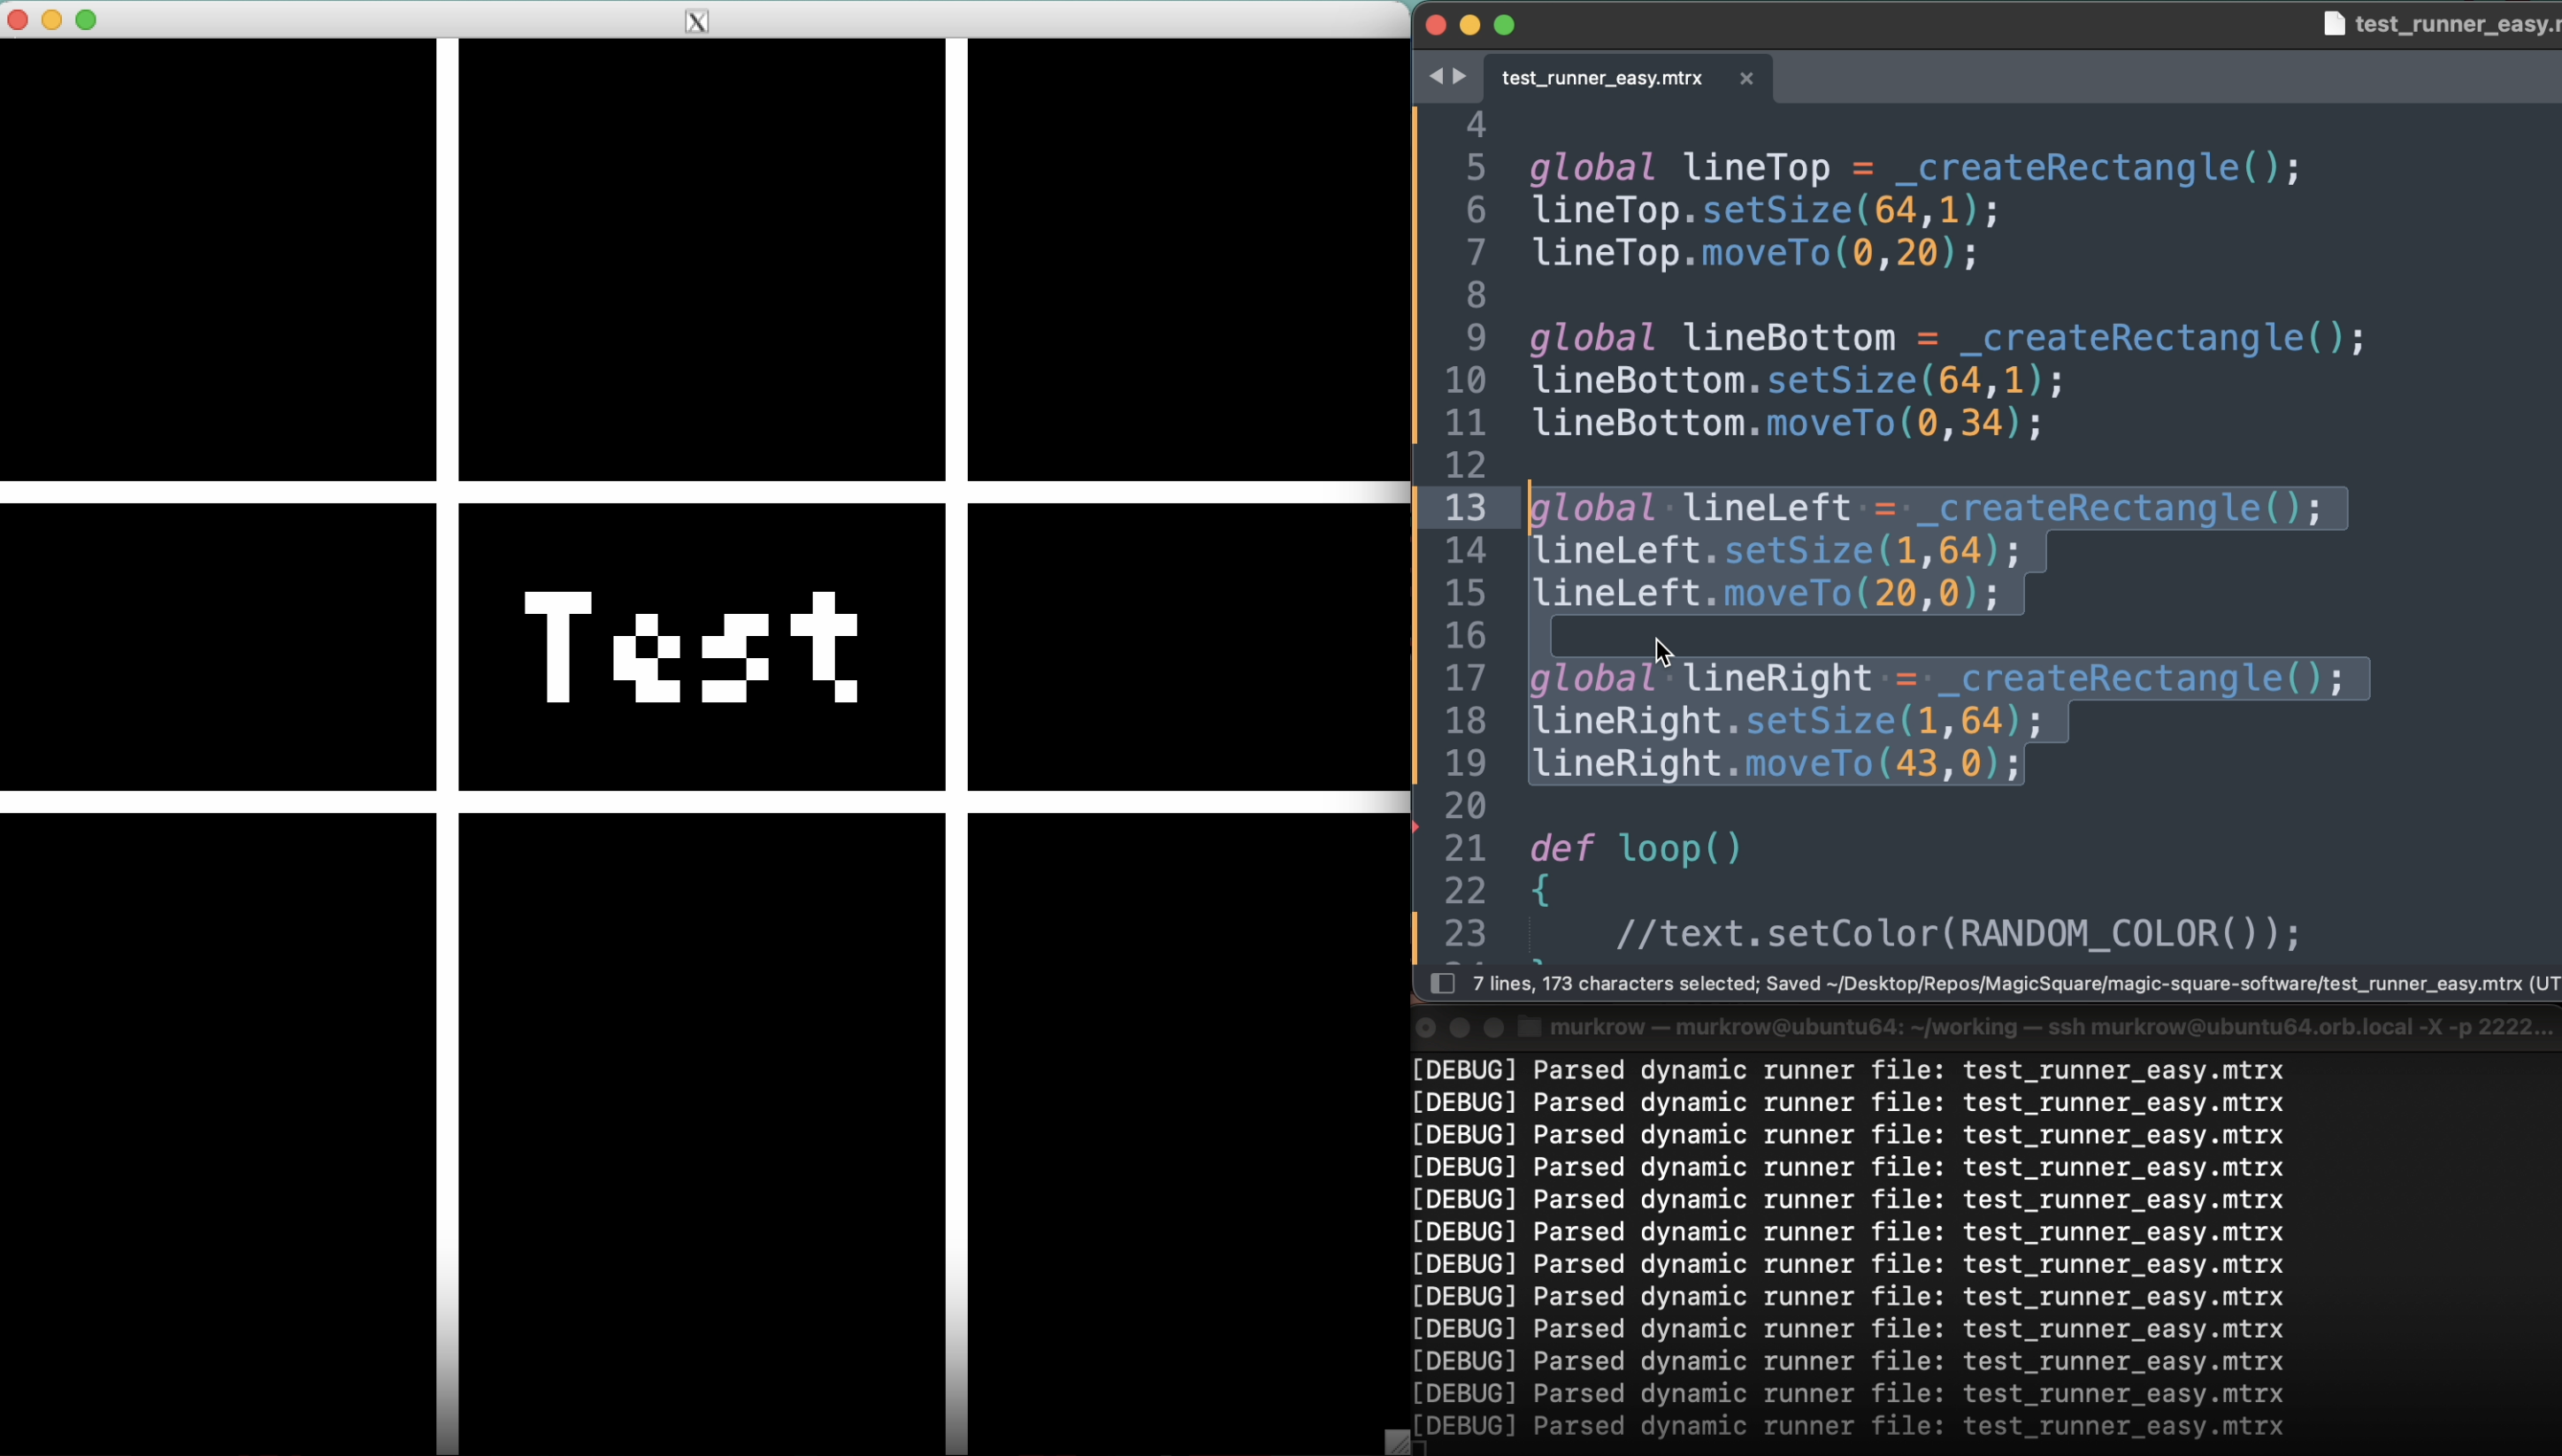
\includegraphics[width=\textwidth]{tesi/img/chai_demo/2.png} \caption*{Creation of 4 rectangles} \end{minipage} \end{figure}

\begin{figure}[h] \centering \begin{minipage}[b]{0.49\textwidth} \centering 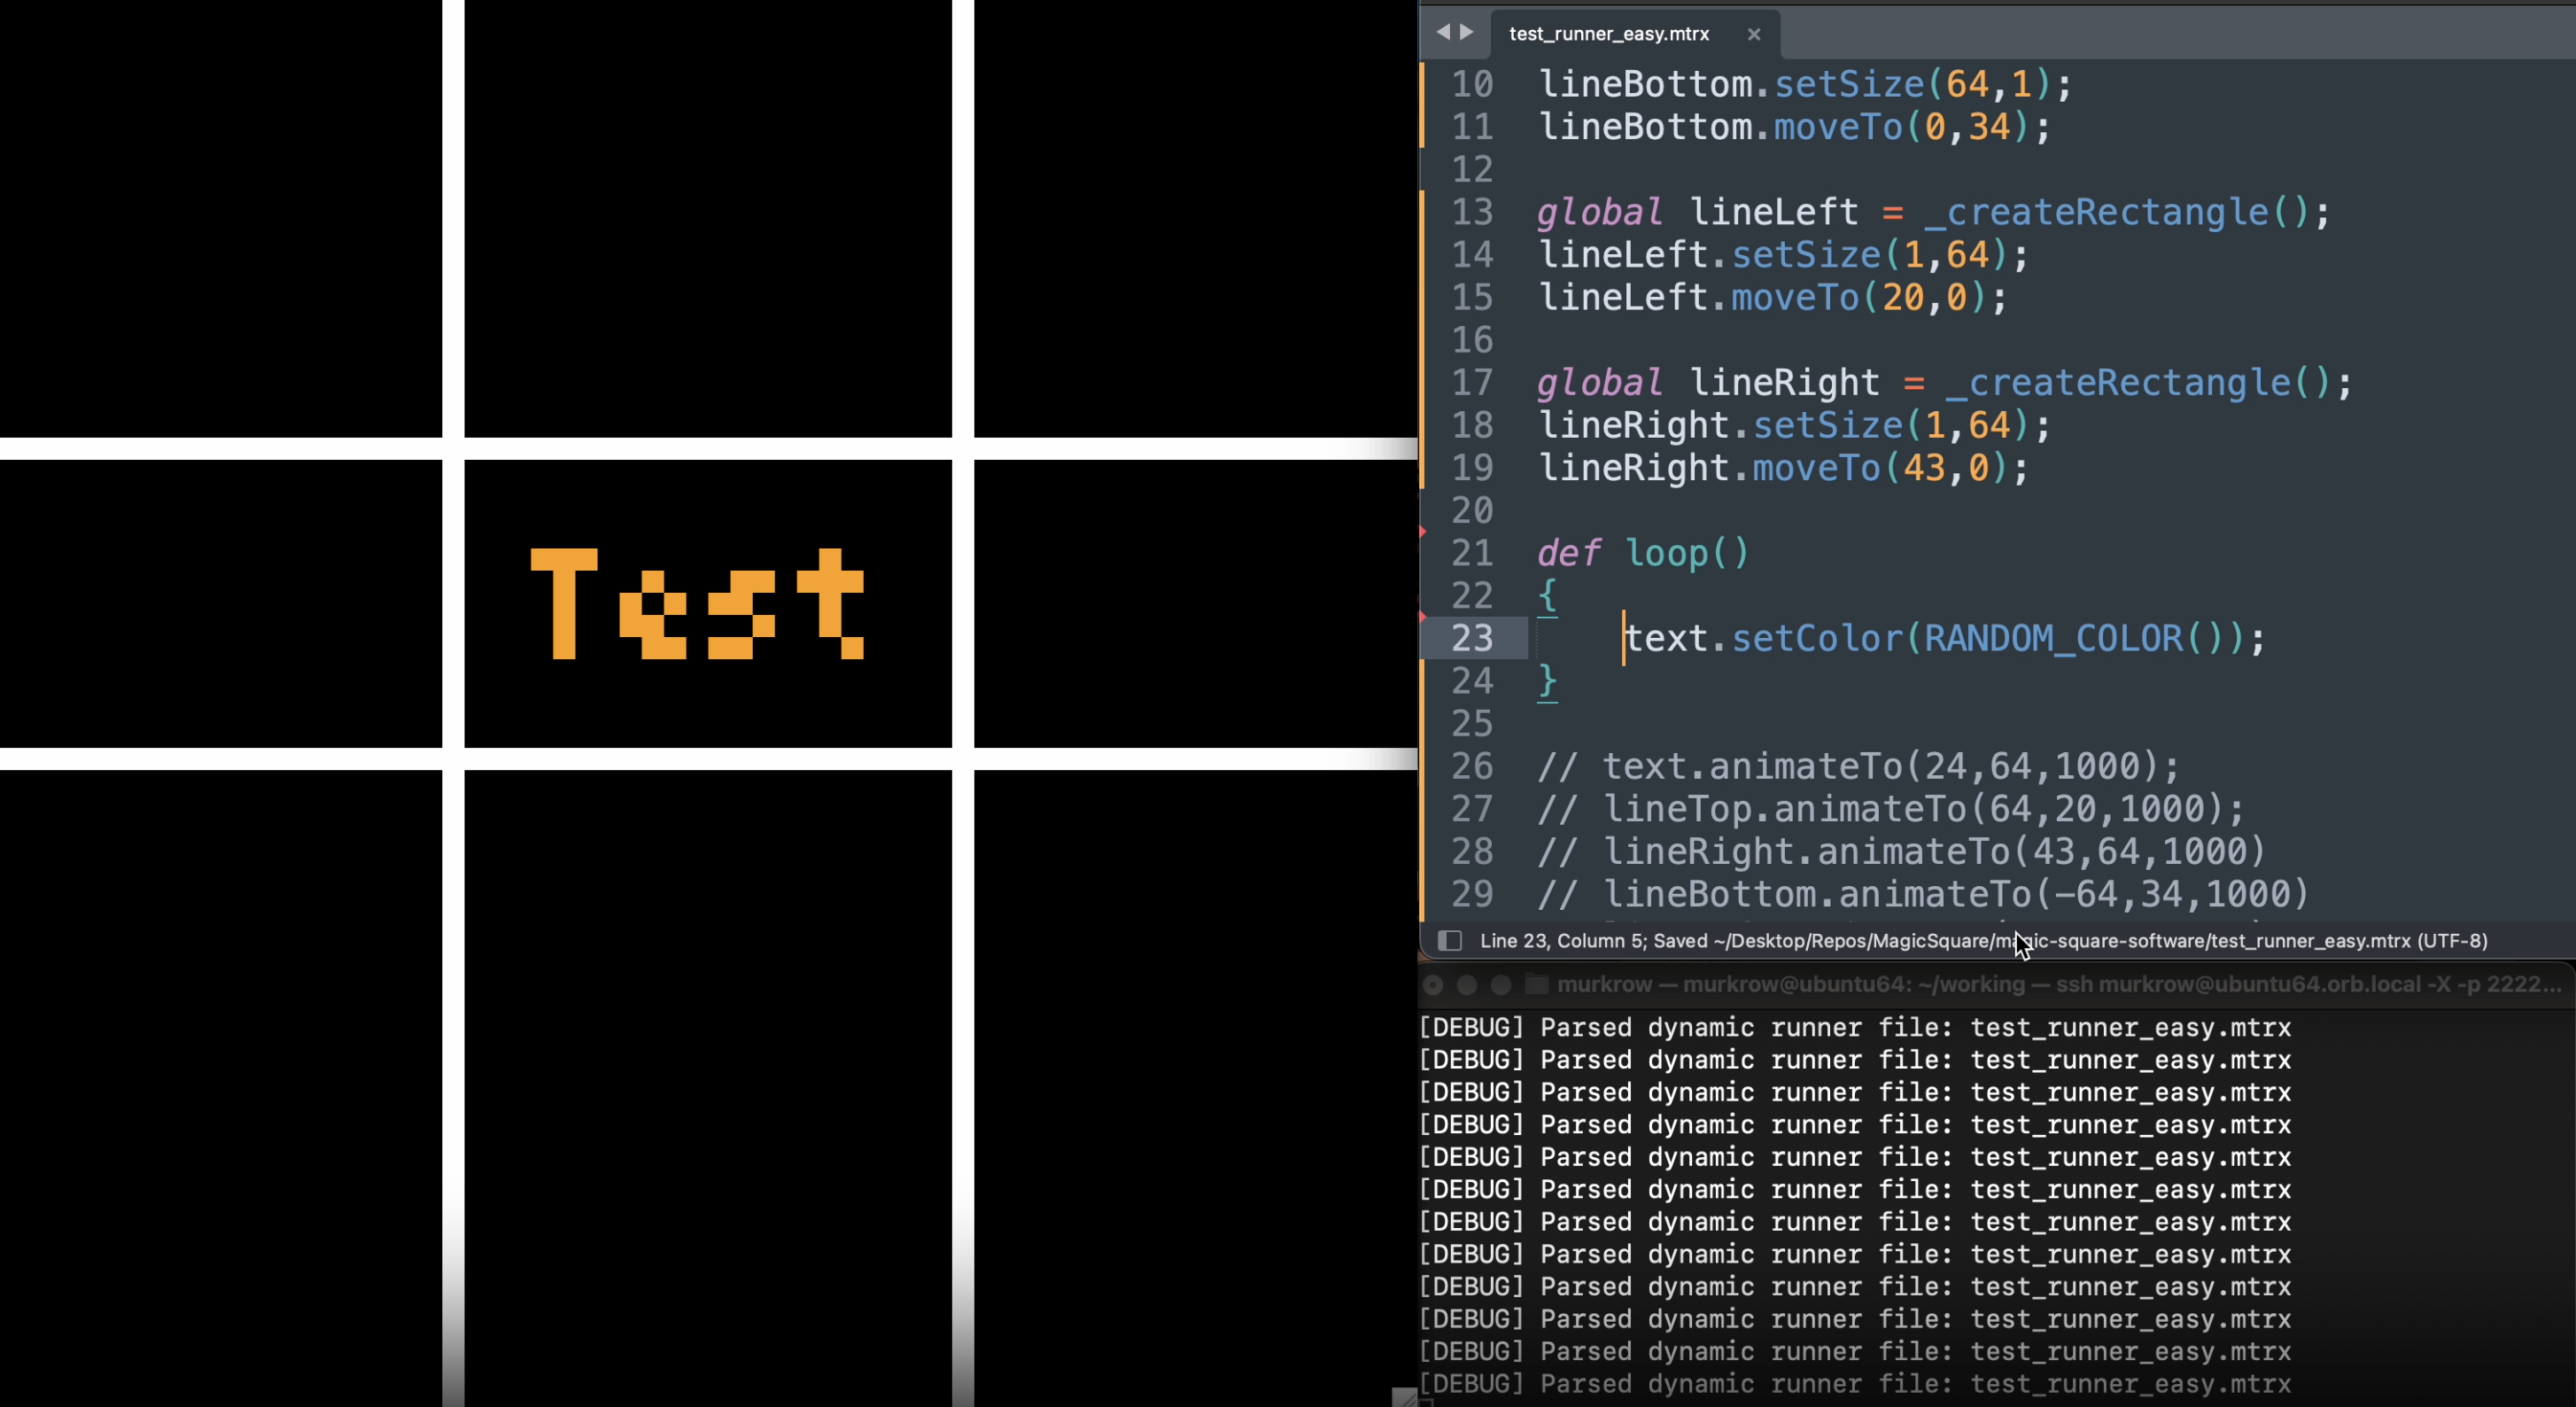
\includegraphics[width=\textwidth]{tesi/img/chai_demo/3.png} \caption*{Set text in random colors in the loop() function} \end{minipage} \begin{minipage}[b]{0.49\textwidth} \centering 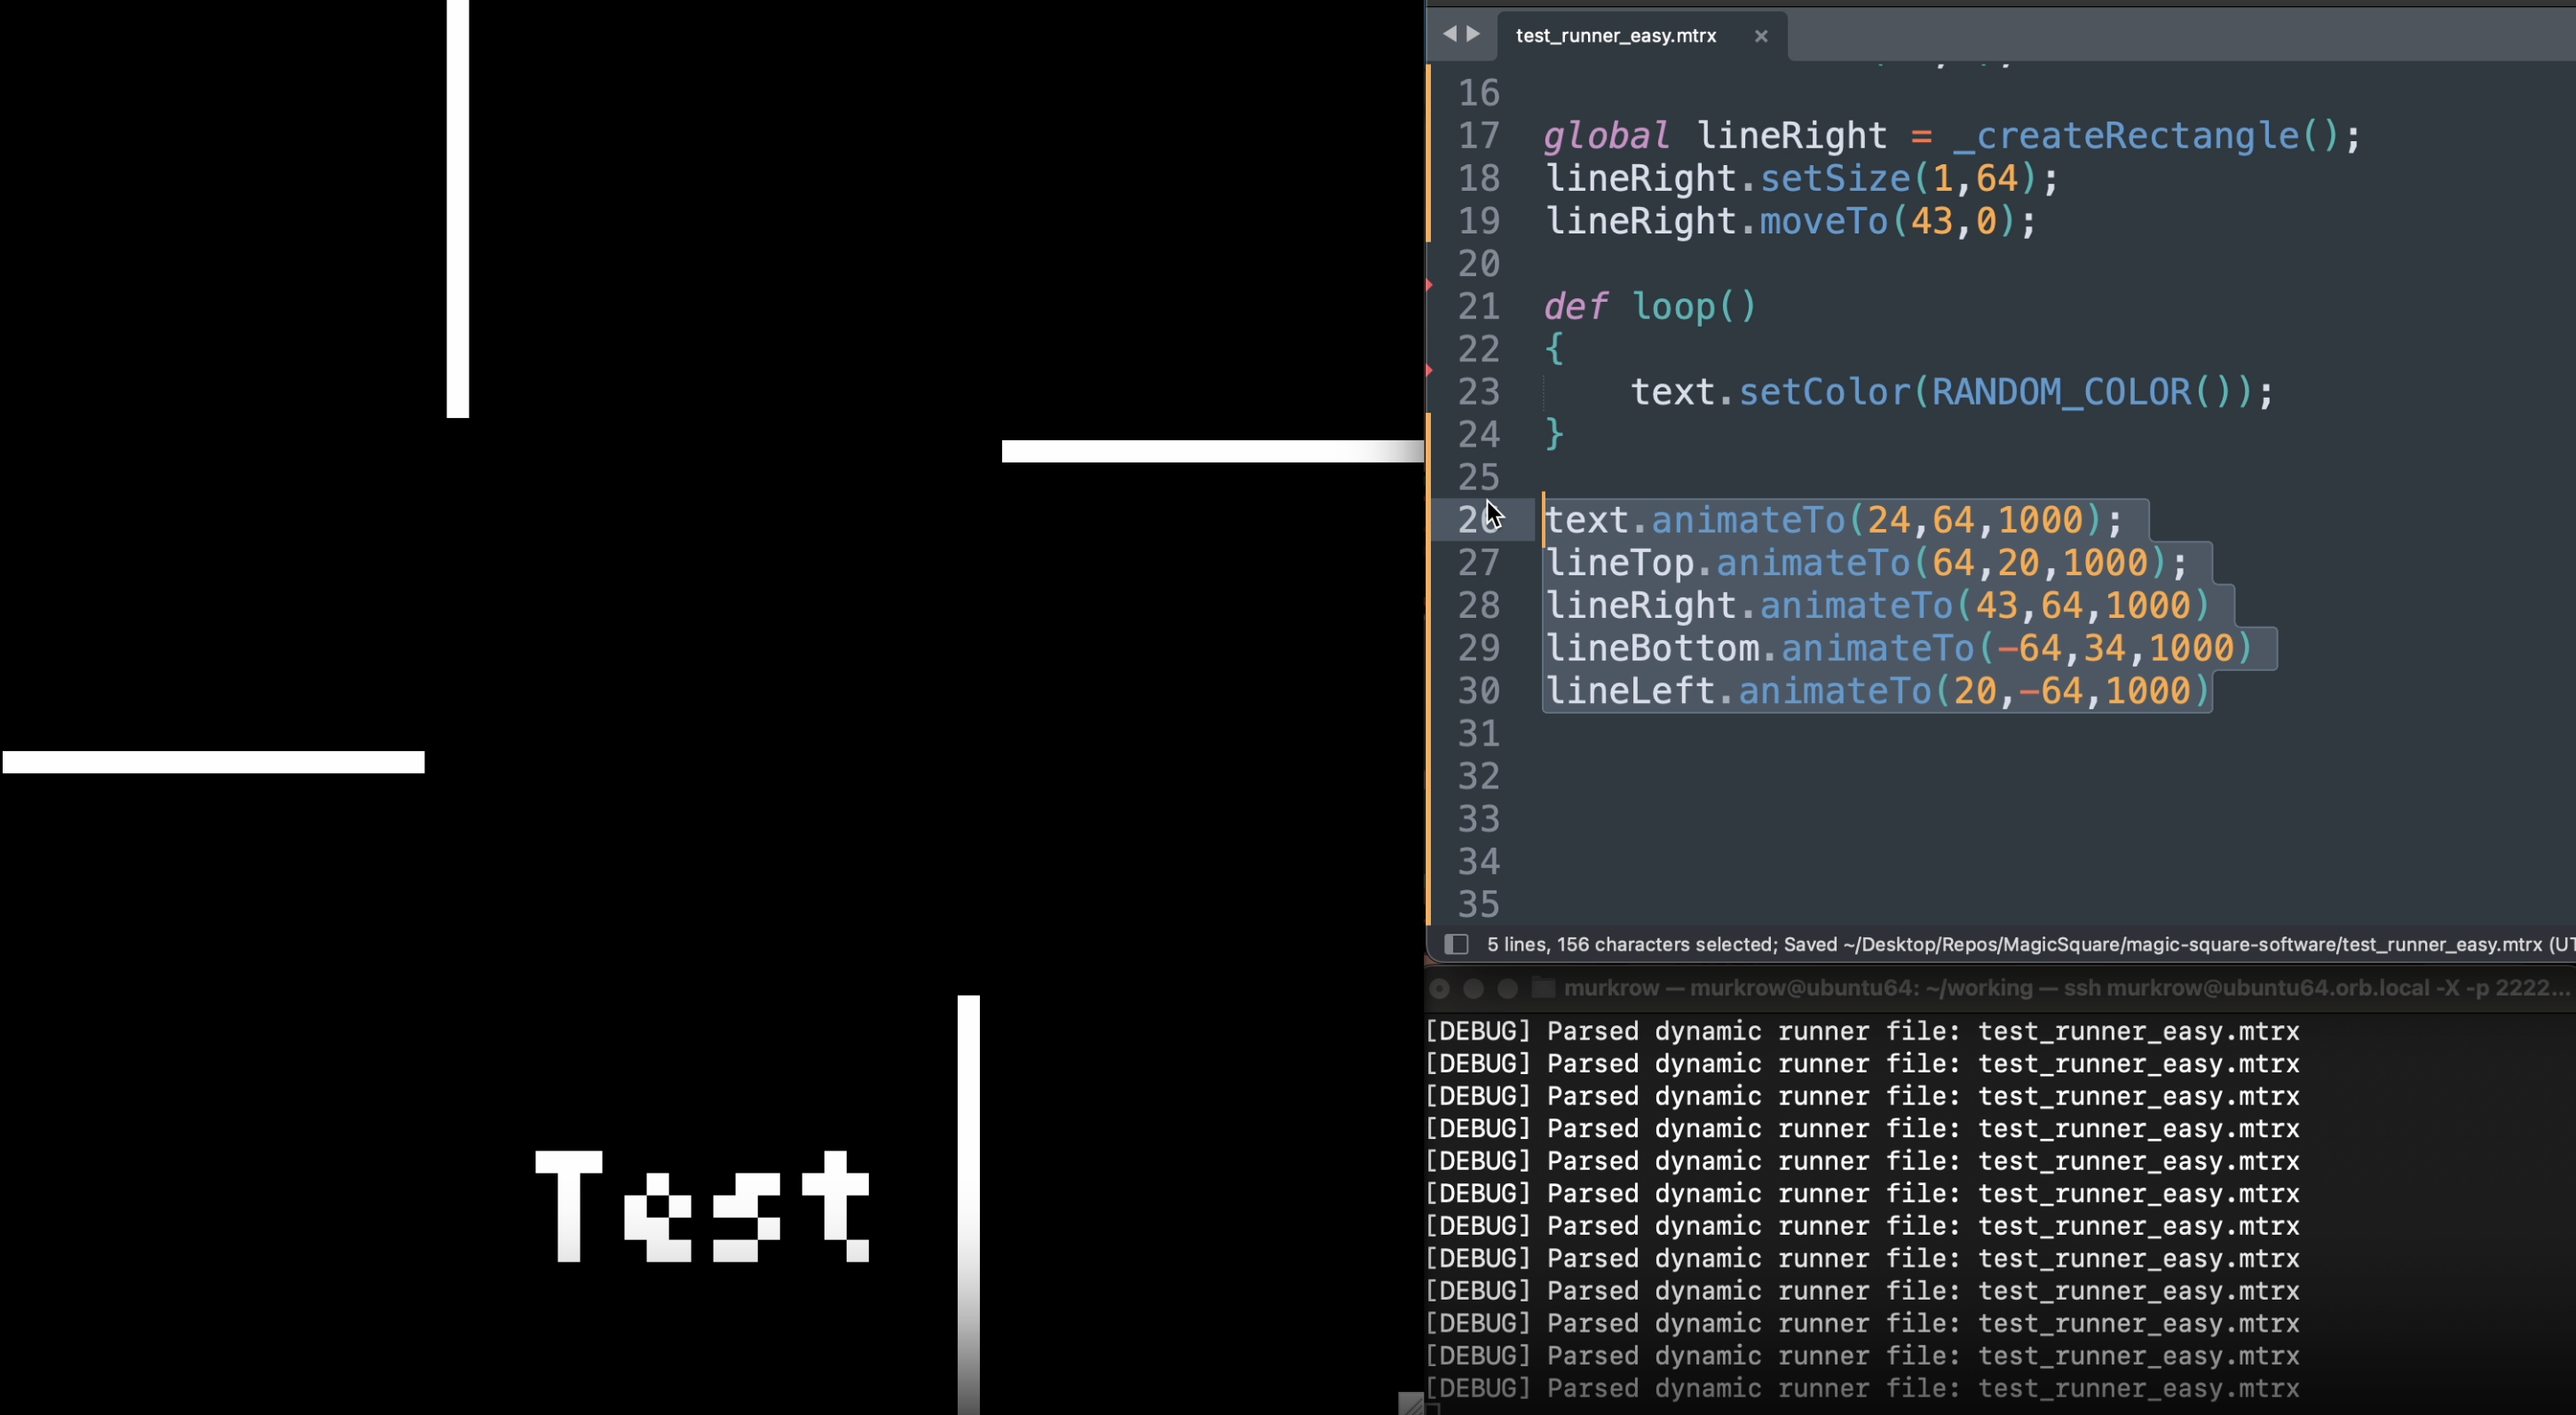
\includegraphics[width=\textwidth]{tesi/img/chai_demo/4.png} \caption*{Animate everything to fade away} \end{minipage} \end{figure}

This solution allowed the engine to interpret and render widgets in real-time, with no recompilation required—an exciting milestone!

\subsubsection{ChaiScript Limitations} While ChaiScript was a solid fit, I eventually realized its limitations:


\begin{itemize}
    \item \textbf{Language popularity}: The language is mostly straightforward and easy to use but is far from being popular. In fact, there are few resources online to learn how to use it, and it's not frequently updated.
    \item \textbf{Language modularity}: Chaiscript has no standard modules. While the community has created a few for tasks such as math functions and JSON deserialization, any additional functionality like a REST client or file management requires wrapping C++ libraries manually.
\end{itemize}


\subsubsection{Discovering Pybind11 and Python Integration} After further research, I discovered Pybind11 \cite{pybind11}, a library that enables seamless embedding of the Python interpreter within C++ code. Despite my initial reservations about Python, its vast modularity—achieved through pip packages—and its popularity made it an attractive alternative to ChaiScript.

With Pybind11, mapping C++ classes to Python objects is nearly effortless, requiring only minimal class declarations. This allowed me to tap into Python's full power while maintaining the performance and flexibility of my C++ engine.


\begin{minted}{c++}
PYBIND11_EMBEDDED_MODULE(mosaico, m) {

    // Bind color class
    py::class_<Color>(m, "Color")
    .def(py::init<int, int, int>());

    // Binding the MatrixWidget class
    py::class_<MatrixWidget>(m, "MatrixWidget")
            .def("createRectangle", &MatrixWidget::createRectangle)
            .def("createImage", &MatrixWidget::createPPM)
            .def("createText", &MatrixWidget::createText)
            .def("createCanvas", &MatrixWidget::createCanvas)
            .def("remove", &MatrixWidget::unregisterDrawable)
            .def("setPixel", &MatrixWidget::setPixel)
            .def("clear", &MatrixWidget::clearDrawables);

    // Bind the Drawable class
    py::class_<Drawable>(m, "Drawable")
    .def("moveTo", &Drawable::moveTo)
    .def("translateBy", &Drawable::translateBy)
    .def("translateXBy", &Drawable::translateXBy)
    // a lot of other stuff
}
\end{minted}

\newpage

The last thing to do is to create a \textit{DynamicWidget} class that will inherit from \textit{Widget} and will invoke the python script to get a new canvas each frame or to register drawables:

\begin{minted}{c++}

class DynamicWidget : public MatrixWidget {
public:
    DynamicWidget(std::string widgetPath, std::string configurationPath){
        // Get files from path and parse metadata
        if (!initializePaths() || !readMetadata()) {
            validWidget = false;
            Logger::logError("Widget initialization failed");
        } else {
            validWidget = true;
            Logger::logDebug("Widget loaded successfully");
        }
        // Register C++ -> Python bindings
        bindObjectsToPython();
        // Load the widget script and execute everything except the loop function
        py::exec(widgetScriptString);
    }
        void renderNextFrame(Canvas* canvas) override {
        try {
            // Execute the loop function
            py::exec("loop()");
        } catch (const py::error_already_set &e) {
            Logger::logError("Error while executing loop function: " + std::string(e.what()));
            validWidget = false;
            canvas->Fill(RED_COLOR);
        }
    }
}
\end{minted}

\newpage

\subsection{Canvas buffer}
The prototype now seems quite ready but there is a single problem left: every widget, even if as far as it is concerned is writing on a \textit{Canvas}, it is still using the real matrix under the hood to render pixels, this can cause problems for scenarios like this:

\begin{minted}{c++}
// Main loop
while (true) {
    matrix->clear();
    // Matrix is full black here
    veryComplexWidget->renderNextFrame(matrix); // will write pixel by pixel
    // Content is now displayed
}
\end{minted}

It is obvious that writing single pixels directly on a matrix is a problem for widgets that requires a bit of computation between pixel and pixel and will result in image flickering.
Luckily the library I used provided me two useful methods:

\begin{minted}{c++}
  // Create a new buffer to be used for multi-buffering. The returned new
  // Buffer implements a Canvas with the same size of thie RGBMatrix.
  // You can use it to draw off-screen on it, then swap it with the active
  // buffer using SwapOnVSync(). That would be classic double-buffering.
  //
  // You can also create as many FrameCanvas as you like and for instance use
  // them to pre-fill scenes of an animation for fast playback later.
  FrameCanvas *CreateFrameCanvas();

  // This method waits to the next VSync and swaps the active buffer with the
  // supplied buffer. The formerly active buffer is returned.
  FrameCanvas *SwapOnVSync(FrameCanvas *other, unsigned framerate_fraction = 1);
\end{minted}

By incorporating these methods into the code, I effectively resolved the flickering issue. This approach enabled smooth rendering by leveraging double-buffering, ensuring that complex widgets could perform the necessary computations without directly writing pixels to the matrix, thus eliminating visual artifacts.

\newpage

I then decided to separate a bit of concerns and I started working on a \textit{CanvasBuffer} class. Since my intent was not to write on the real matrix anymore but to create a set of canvas to swap on the matrix at some point in time, I also seized the occasion to make these canvases even more generic by giving them the possibility to be of arbitrary sizes, they still needed to be smaller than the hardware matrix itself but they could occupy for example the bottom half of the screen, the top left quarter etc. I called this class \textit{CanvasLayer} and it looks like this:

\begin{minted}{c++}
/// A CanvasLayer is a layer that can be painted on by a widget.
/// Allows to create composite widgets to be displayed on the matrix.
/// Can be narrower or shorter than the matrix.
class CanvasLayer : public Canvas {

private:

    // Pixels are stored in a list to allow for 
    // easy iteration and manipulation
    std::list<Pixel> pixels;

public:

    CanvasLayerPosition pos;
    CanvasLayer(CanvasLayerPosition position = CanvasLayerPosition::FULL);
    ~CanvasLayer();

    // Will actually write pixels on another canvas (even the matrix)
    void paintOntoCanvas(Canvas *canvas, int xOff = 0, int yOff = 0);
    int width() const;
    int height() const;
    void Fill(Color color);
    void SetPixel(int x, int y, Color color);
    void Clear();
    CanvasLayer *Clone();
    void setBorder(Color color);
    void setPadding(int padding);
    int getPixelCount();
};
\end{minted}

\newpage

As you may notice, the \textit{CanvasLayer} class simply implements the \textit{Canvas} interface. The principle of dependency inversion mentioned before \ref{widget_canvas_abstraction} allowed me to do this upgrade while being completely transparent to objects that worked with a \textit{Canvas}.

This is what the \textit{CanvasBuffer} class looked like:


\begin{minted}{c++}

/// This class is responsible for buffering the canvas frames
/// This is useful when you want to render multiple widgets on the matrix and be able to show them all at once
/// The buffer will be able to swap the frames on the matrix without flickering
class CanvasBuffer {

private:
    MatrixDevice *matrix;
    std::list<Canvas*> buffer;

public:
    CanvasBuffer(MatrixDevice *matrix, int bufferSize) {
        this->matrix = matrix;
        for (int i = 0; i < bufferSize; i++) {
            buffer.push_back(matrix->CreateFrameCanvas());
        }
    }
    // This can be called multiple time for the current frame
    // Is basically used to compose the final composite frame
    // to later swap on the matrix using loadNextFrameOnMatrix()
    void paintPartialLayerOnCurrentFrame(CanvasLayer *canvasLayer) {
        auto *currentFrame = buffer.front();
        canvasLayer->paintOntoCanvas(currentFrame);
    }
    // Uses the frame crafted with the method above to swap it on actual matrix
    void loadNextFrameOnMatrix() {
        // Swap current frame on matrix
        auto *currentFrame = buffer.front();
        buffer.pop_front(); 
        matrix->SwapFrameCanvas(currentFrame); 
        buffer.push_back(currentFrame); 
        // Prepare next frame
        auto *nextFrame = buffer.front();
        nextFrame->Clear();
    }
};
\end{minted}

\newpage
This is the high-level view of the whole final rendering software:

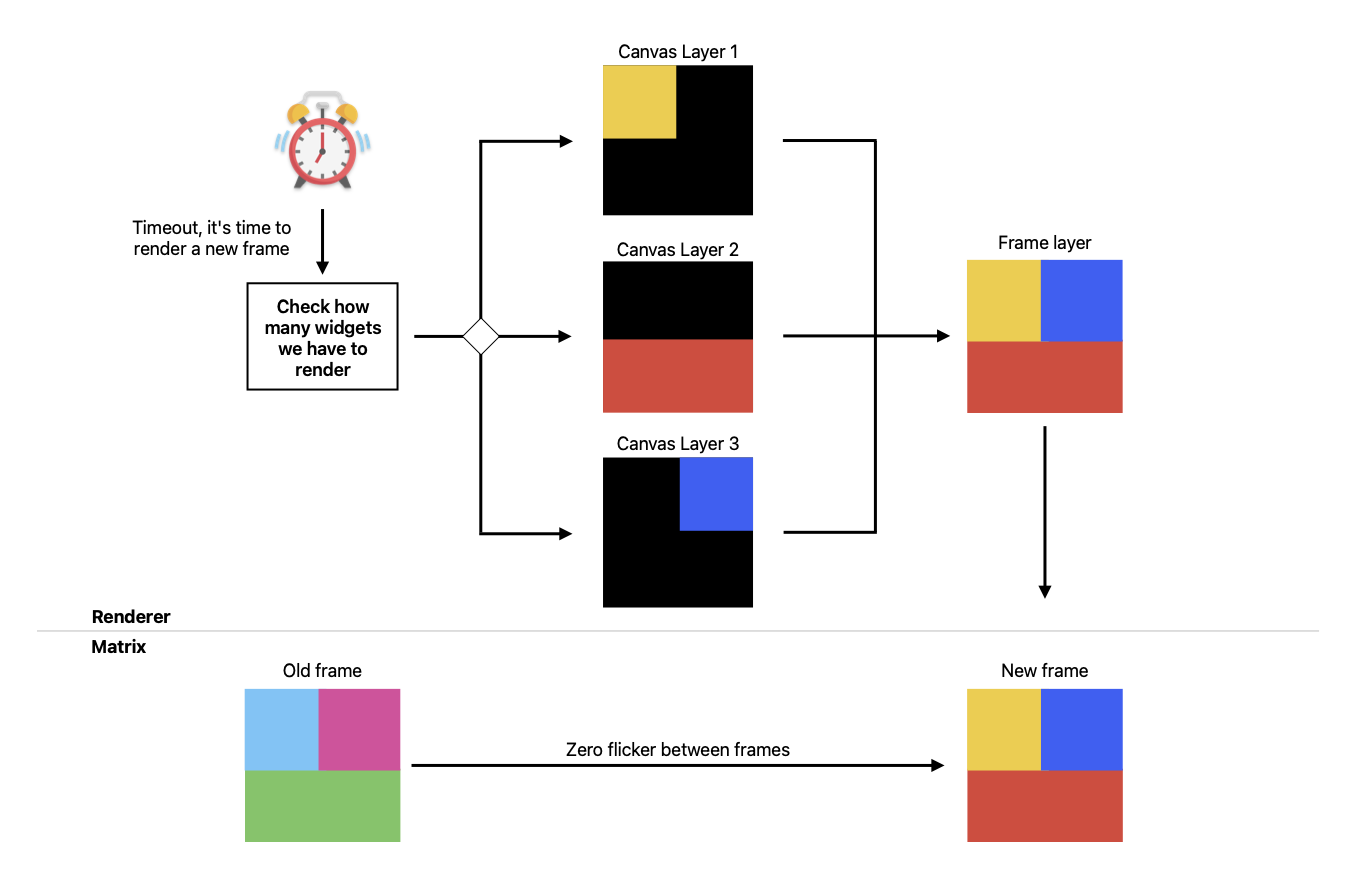
\includegraphics[width=\textwidth]{tesi/img/software-renderer.png}
\newpage
\section{Python Module}
Initially, my intention was to develop the entire software in C++. However, it became evident that a significant amount of time was being wasted on implementing basic functionalities, such as making remote API calls, deserializing JSON objects, or managing simple data in a local SQLite database.

As I have grown accustomed to working with higher-level abstractions that facilitate productivity and enable the maintenance of clean, organized codebases, it became apparent that achieving similar levels of efficiency in C++—a language not primarily designed for such tasks—was considerably more challenging. 

The complexity escalated when I attempted to set up a BLE GATT (Bluetooth Low Energy Generic Attribute) server in C++. I discovered that no high-level abstractions existed for this purpose in any of the available C++ libraries. In contrast, I found an easy-to-use and powerful Python library called \textit{Bless}\footnote{\url{https://pypi.org/project/bless/}}.

This realization led me to a pivotal decision: to shift the networking and data management logic from C++ to Python, thereby leveraging Python's simplicity and robust ecosystem. This move allowed the C++ module to focus on a single, well-defined responsibility: rendering pixels and handling graphics efficiently.

The Python module is designed to serve three primary purposes:
\begin{itemize}
    \item Enable auto-discovery of the matrix for the client application via BLE.
    \item Establish a lightweight LAN COAP server to receive and process commands from the client app.
    \item Manage persistent data, such as user-specified widget configurations using a simple relational SQLite database.
\end{itemize}

\newpage
To facilitate communication between the C++ and Python modules, I implemented a Unix socket, allowing seamless inter-process communication between the two languages.

This is a complete specification of the possible commands that the COAP server can receive:

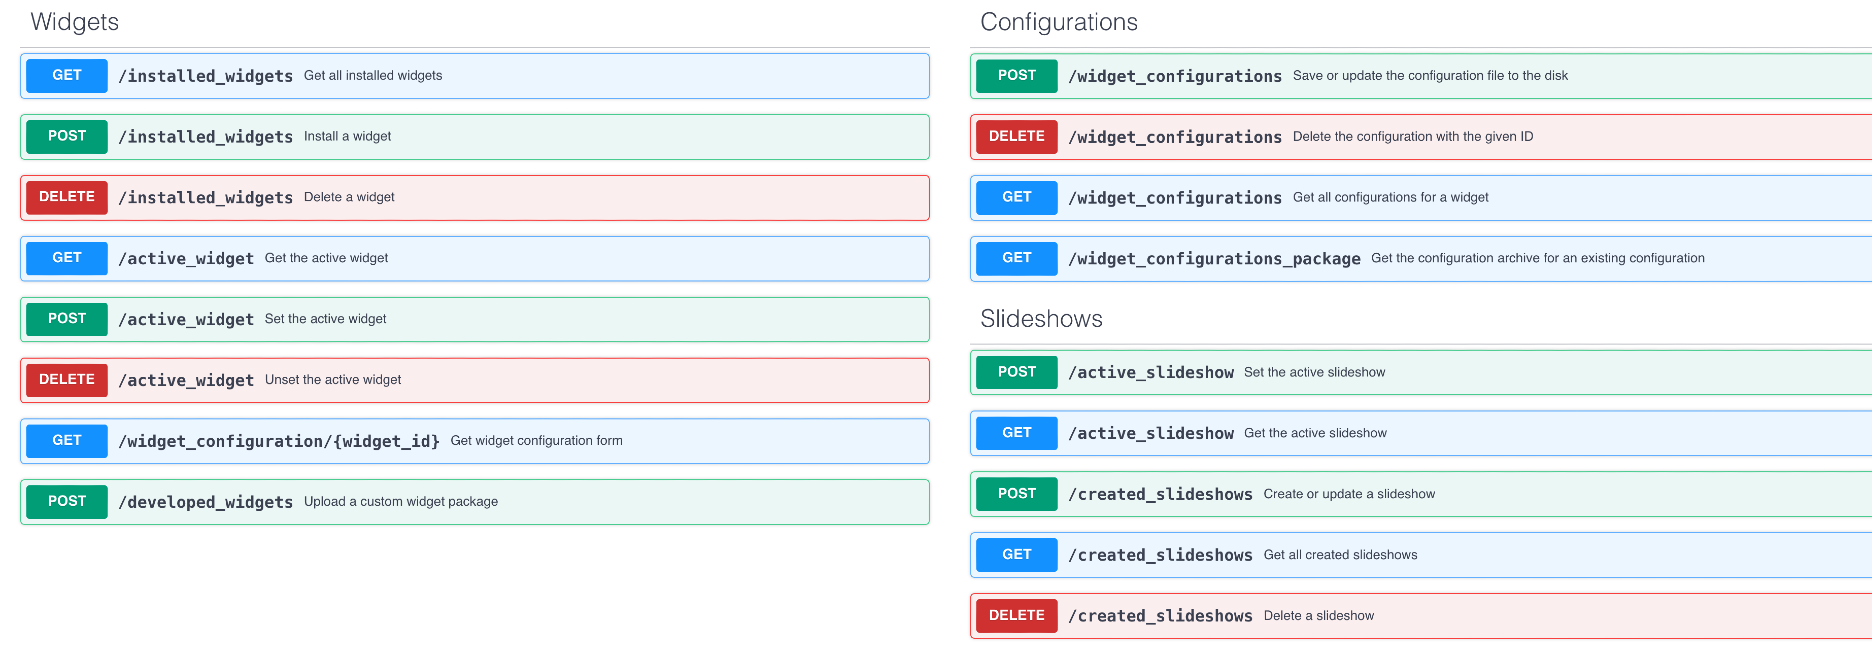
\includegraphics[width=1\textwidth]{tesi/img/coap-swagger.png}

This is an example interaction between the user, the app, the Python module and the C++ module:

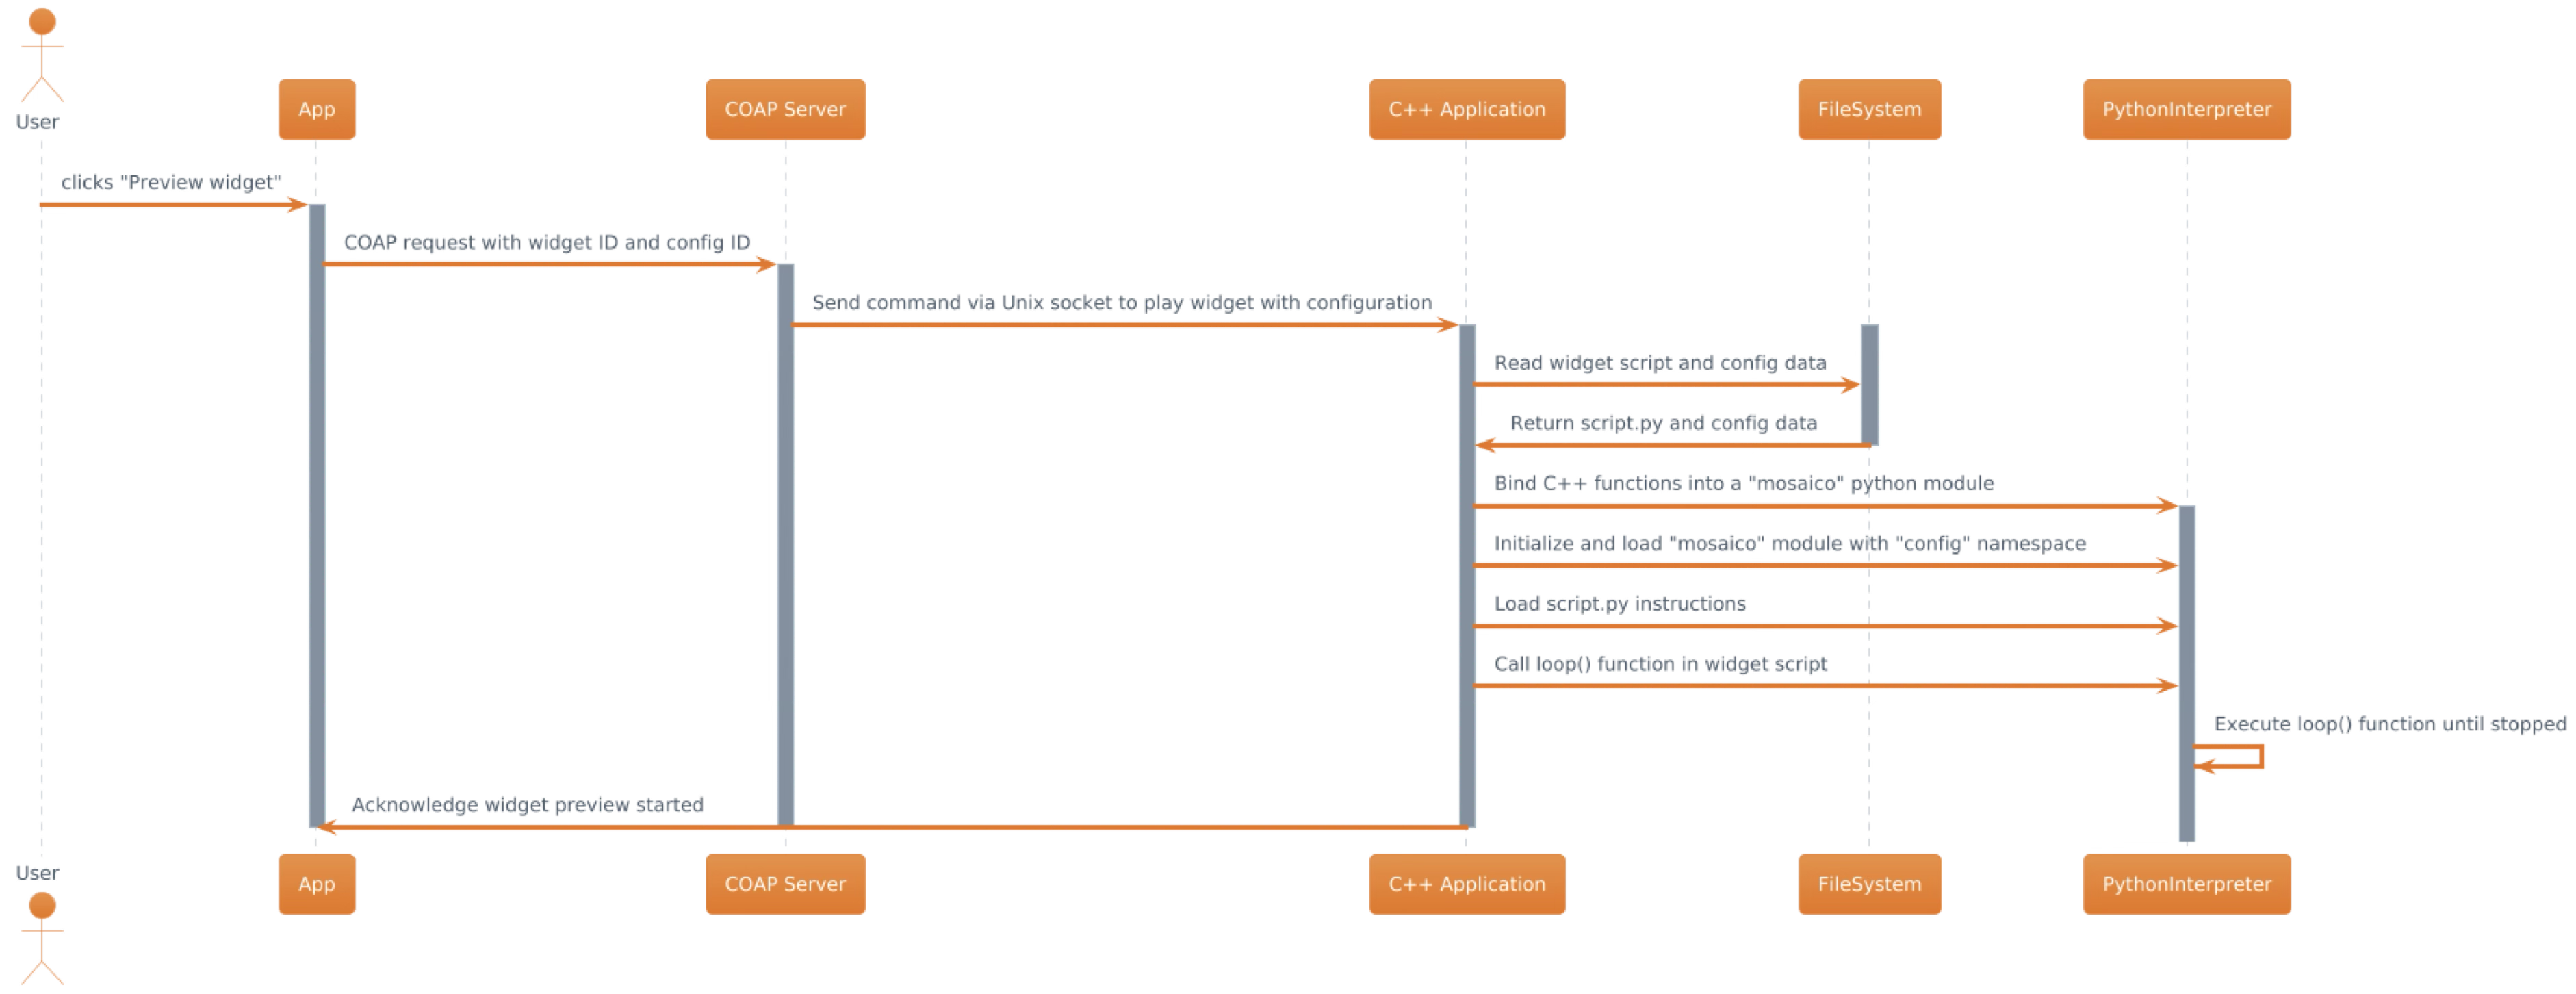
\includegraphics[width=1\textwidth]{tesi/img/activity-install-widget.png}
\newpage
\section{Cross Compiler}
One of the more challenging aspects of developing a complex C++ application is the creation of a makefile that accurately links all required modules and libraries. This challenge becomes even more pronounced when targeting a different architecture, as in the case of compiling for the ARMv6 CPU of the Raspberry Pi Zero W.

Compiling directly on the Raspberry Pi proved impractical, as each compilation took between 10 to 20 minutes to generate an executable—an unacceptable delay for iterative development. 

After extensive experimentation, I successfully identified a working cross-compilation toolchain tailored to the ARMv6 architecture \footnote{\url{https://github.com/tttapa/docker-arm-cross-toolchain/}}. This discovery significantly optimized the build process, reducing compile times to less than a minute. To streamline the development workflow, I created a Bash script that automates the compilation, establishes an \textit{SSH} connection to the Raspberry Pi, and uses \textit{rclone} to swiftly transfer the build artifacts to the device before launching the application.

Though this setup took considerable time to establish, it drastically accelerated the development process, allowing for rapid testing and debugging on the Raspberry Pi.

\newpage
\section{Simulators}
\label{simulators}
\begin{figure}[h]
 \centering
 \begin{minipage}[b]{0.32\textwidth}
    \centering
    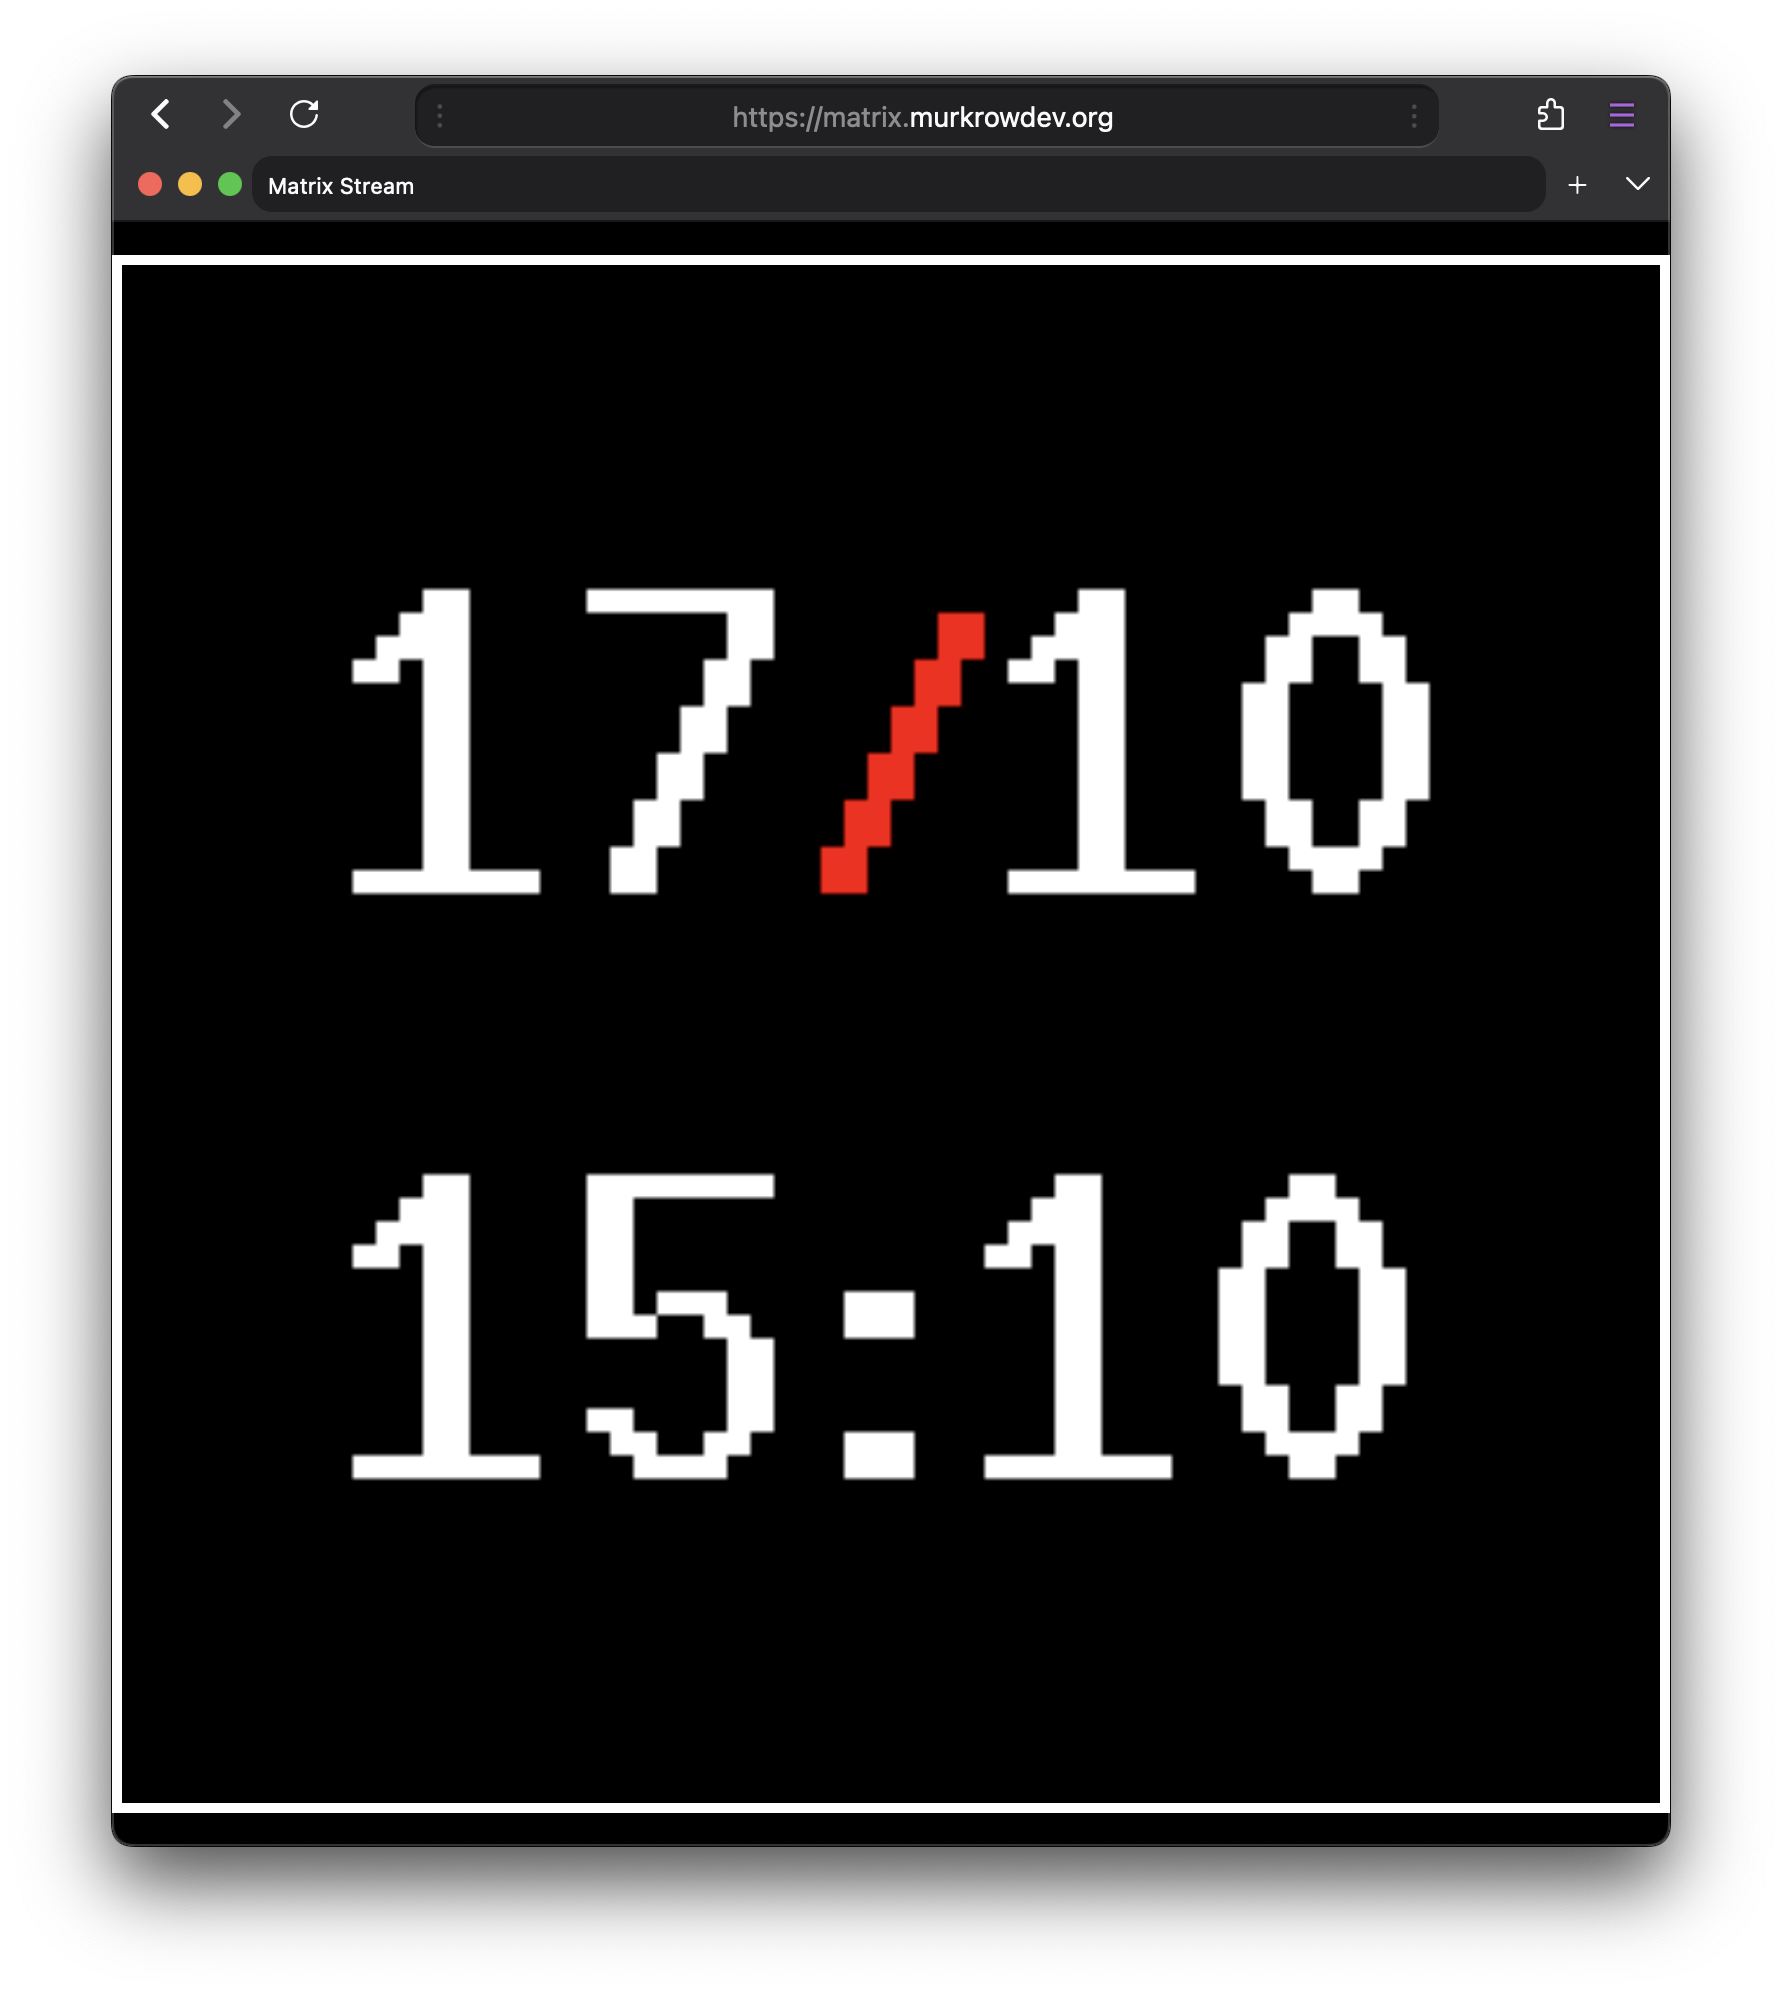
\includegraphics[width=\textwidth]{tesi/img/matrices/web.png}
    \caption*{Web simulator}
\end{minipage}
    \centering
    \begin{minipage}[b]{0.32\textwidth}
        \centering
        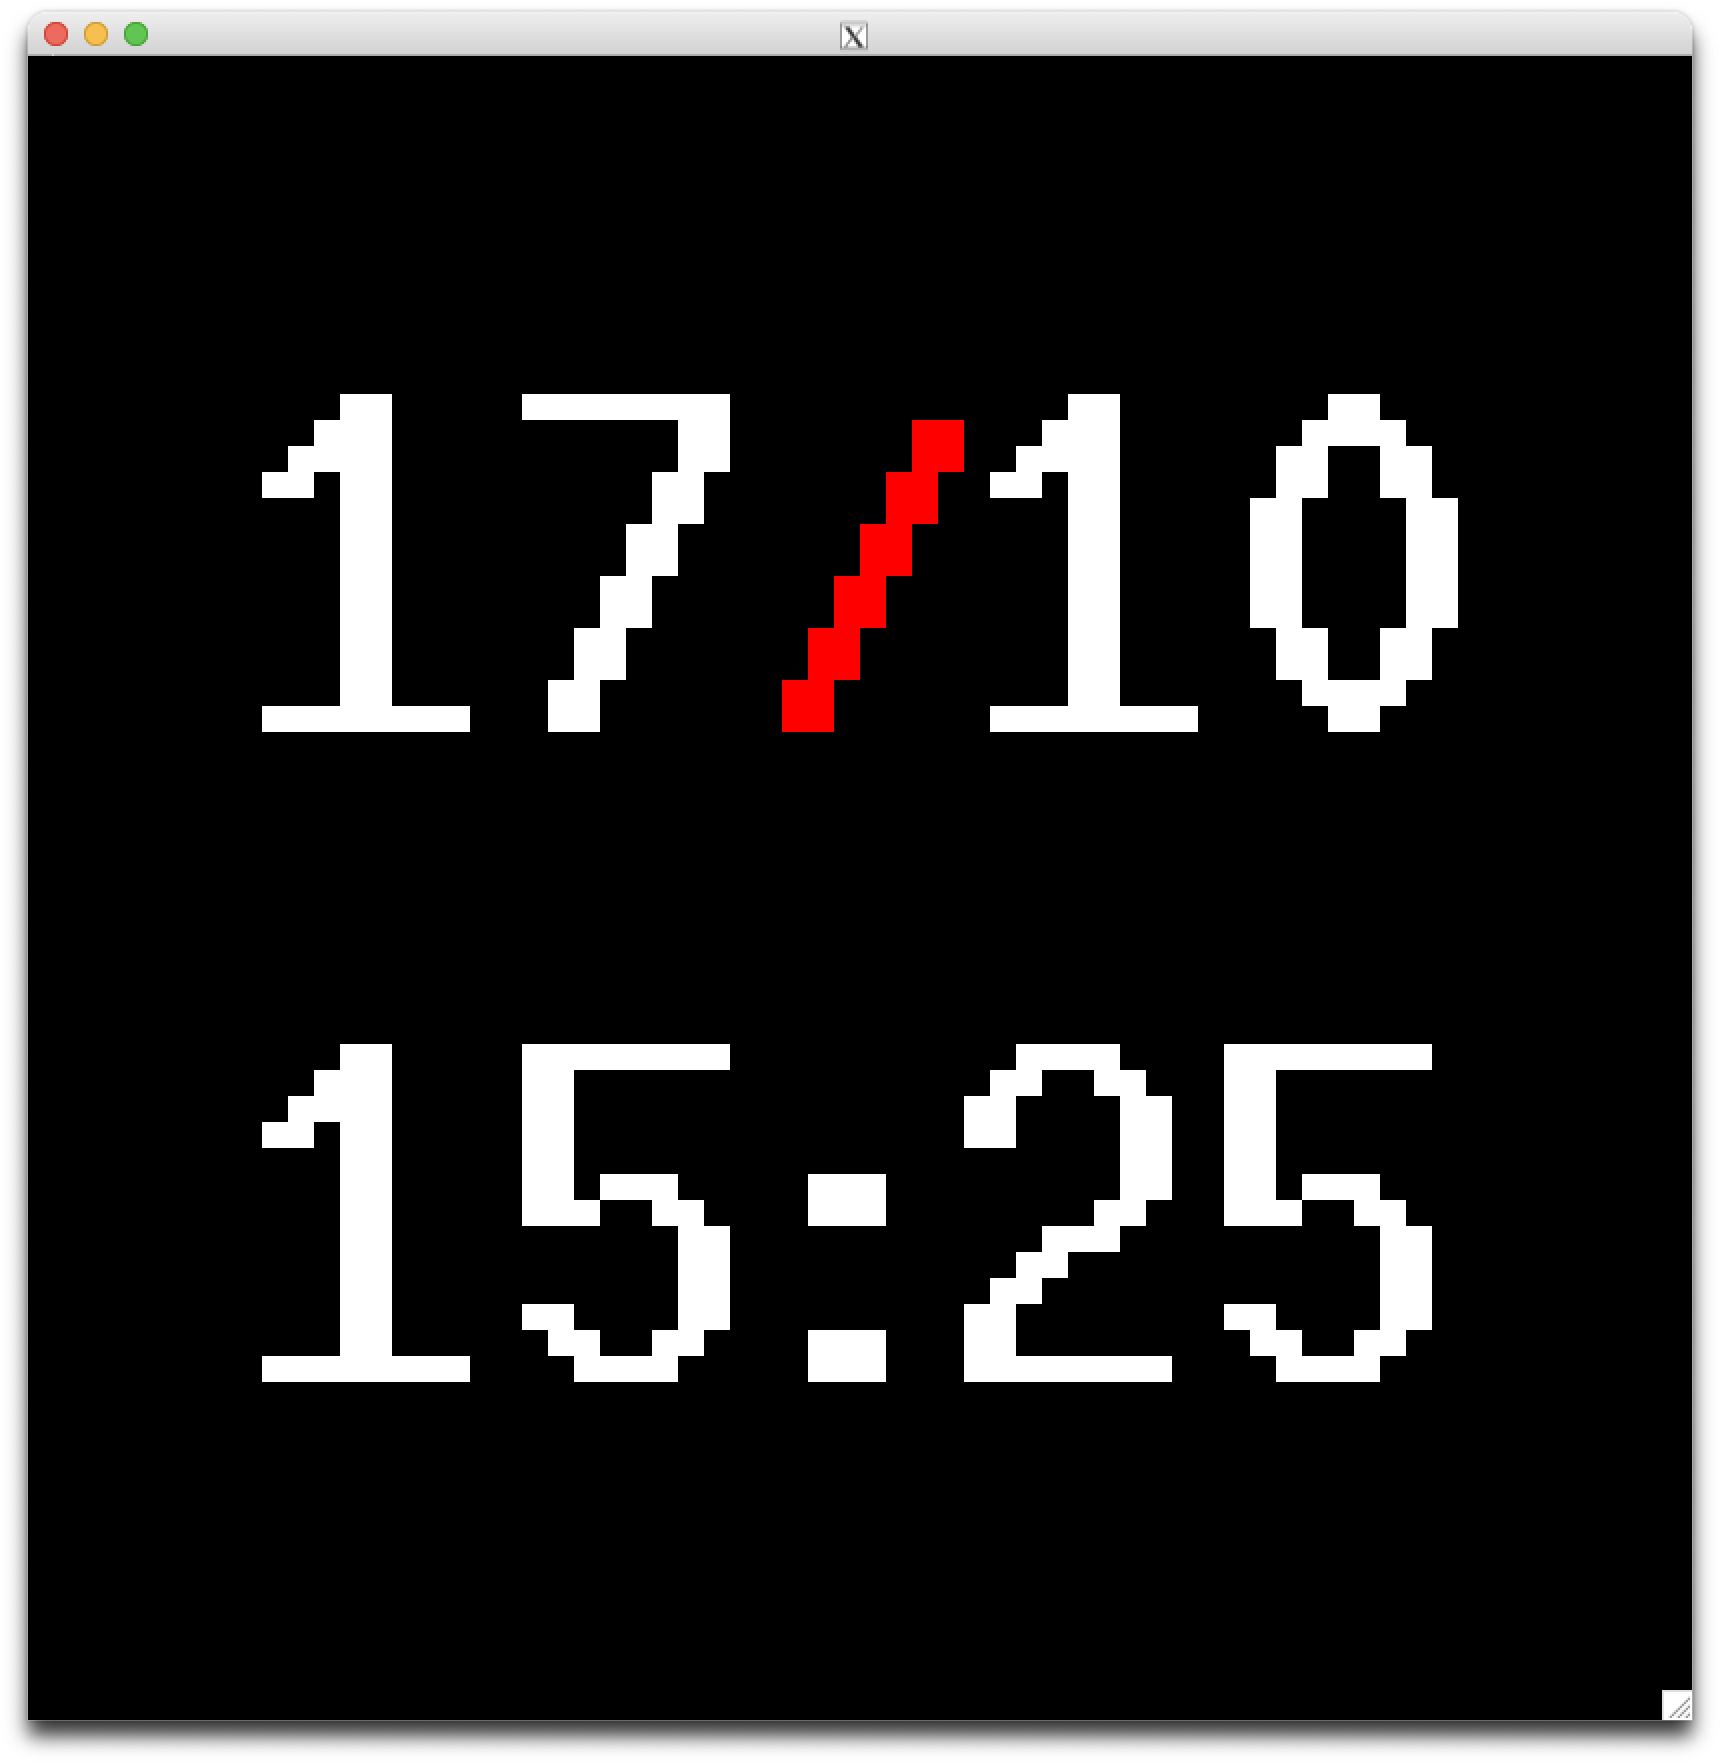
\includegraphics[width=\textwidth]{tesi/img/matrices/x11.png}
        \caption*{X11 windowed simulator} 
    \end{minipage}
    \centering
    \begin{minipage}[b]{0.32\textwidth}
        \centering
        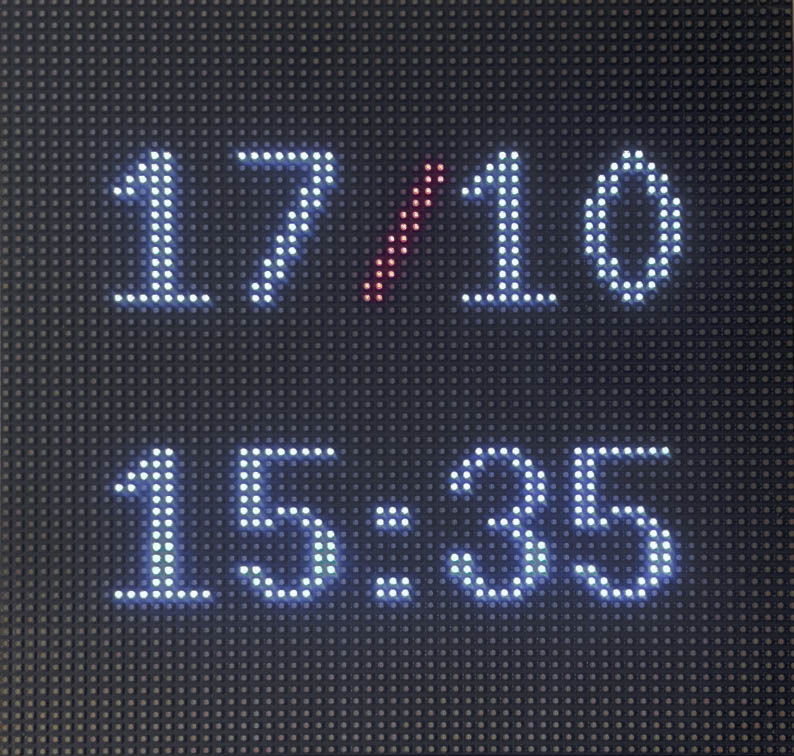
\includegraphics[width=\textwidth]{tesi/img/matrices/real.jpg}
        \caption*{Real matrix} 
    \end{minipage}
\end{figure}


Even with cross-compilers meticulously configured, the process of compiling and syncing files continued to be a significant drain on development time. Furthermore, given that I am frequently away from home, I sought a solution that would allow me to work on the project remotely, without the need for the physical hardware. Clearly, carrying the matrix and Raspberry Pi with me at all times was not a practical option. This led me to explore the idea of developing a matrix simulator from scratch.

Initially, the task appeared daunting, as I anticipated that a substantial amount of time and effort would be required to implement such a simulator. However, once again, the design principles employed throughout the application—particularly the use of dependency inversion—proved to be immensely beneficial.

One of the key architectural decisions in the project was to ensure that, aside from the application’s entry point, no other modules would have direct knowledge of the matrix hardware. Instead, all modules interact with a generalized abstraction—a \textit{Canvas} interface. This meant that, in order to implement the simulator, I only needed to create a new class that conformed to the \textit{Canvas} interface, and dynamically switch between the actual hardware matrix and the simulator based on specific conditions.

These conditions were introduced through a pre-processor argument passed during the compilation process, enabling the system to determine whether to instantiate the actual hardware or the simulated matrix. Subsequently, I modified the main application logic to utilize a \textit{MatrixBuilder} class, which abstracts the creation of the matrix, making it agnostic to the specific implementation (hardware or simulation). The \textit{MatrixBuilder} class is a simple factory that returns a \textit{MatrixDevice} object, based on the conditions provided during compilation.

\begin{minted}{c++}
class MatrixBuilder
{
public:
    static MatrixDevice* build()
    {
#if SIMULATION
        return new X11Matrix();
#elif WEB
        return new MatrixStream();
#else
        return new HardwareMatrix();
#endif
    }
};
\end{minted}

The output of the \textit{MatrixBuilder} is a \textbf{MatrixDevice} object, which is a custom class I developed to encapsulate the various matrix implementations. This wrapping was necessary because the matrix class provided by the library could not be directly modified. Thus, I introduced a custom class to act as an intermediary, wrapping the existing library class.

\begin{minted}{c++}
class HardwareMatrix : public MatrixDevice {
private: RGBMatrix *matrix;
public: 
HardwareMatrix() {

    // Configure the RGBMatrix
    RGBMatrix::Options matrix_options;
    rgb_matrix::RuntimeOptions runtime_opt;

    // Create the RGBMatrix object
    RGBMatrix *matrix = RGBMatrix::CreateFromOptions(matrix_options, runtime_opt);
    this->matrix = matrix;
}
Canvas* CreateFrameCanvas()
{
    return matrix->CreateFrameCanvas();
}
void SwapFrameCanvas(Canvas *canvas){
    matrix->SwapOnVSync((FrameCanvas*)canvas);
}
}; \end{minted}

This design provided the necessary flexibility, allowing me to switch between different matrix implementations without significant modifications to the underlying logic. The use of a wrapper class ensured compatibility with the existing library while offering the opportunity to extend functionality when necessary.

\subsection{The X11 Simulator}

The X11-based simulator serves as a graphical approximation of the actual matrix hardware. By leveraging the X11 windowing system, it simulates the behavior of the matrix display in a window on the desktop environment, replicating the visual effects and behavior of the matrix as a 1:1 replica of the original. This is the actual simulator I used while developing the application since is the better performing one.

\subsection{The Web Simulator}
\label{web-simulator}
The web-based simulator provides a more accessible, platform-independent alternative, allowing users to interact with the system remotely. It is composed of two main components: a C++ module responsible for rendering frames, which serializes them as an array of RGB values and transmits them through a UNIX socket, and a Python server built with Flask. The Flask server receives the data, processes it, and transmits it in real-time via WebSockets to an HTML page, also served through Flask, where the live stream is rendered for users to interact with.

This design offers real-time simulation capabilities and enables users to experience the system without the need for physical hardware. A publicly accessible instance of this simulator has been deployed to allow users to test Mosaico, available at \url{https://matrix.murkrowdev.org/}.

